\section*{Chapitre 1 - Activité 1 : Découverte de la distributivité}

\subsection*{Découverte par quinze}

\cnt Calculer $8\times (10+5)$ et $8\times 10 + 8 \times 5$. Que remarque-t-on ?

\cnt Calculer $7\times (10+5)$ et $7\times 10 + 7 \times 5$. Que remarque-t-on ?

\cnt En déduire une technique rapide pour multiplier un nombre par 15.

\cnt Effectuer les calculs suivants :

\begin{multicols}{4}
    $3\times 15$

    $11\times 15$

    $20\times 15$

    $50\times 15$
\end{multicols}

\subsection*{Approche géométrique}

On considère la figure ci-dessous composée des rectangles $BCDE$ et $ABEF$.



\begin{minipage}[m]{0.35\textwidth}
    \begin{figure}[H]
        \centering
        \begin{tikzpicture}
            \draw (0,0) node [below] {$A$}--(3,0) node [below] {$B$}--(5,0) node [below] {$C$}--(5,2.5) node [above] {$D$}--(3,2.5) node [above] {$E$}--(0,2.5) node [above] {$F$}--cycle;
            \draw (3,0)--(3,2.5);
        \end{tikzpicture}
    \end{figure}
\end{minipage}
\hfill
\begin{minipage}[m]{0.6\textwidth}
    Pour $AB=10$, $BC=2$ et $AF=7$ :
    
    \cnt Calculer l'aire de $ABEF$
    
    \cnt Calculer l'aire de $BCDE$
    
    \cnt Calculer l'aire de $ACDF$ de deux manières différentes.
    
    \cnt Même question pour $AB=20$, $BC=4$ et $AF=8$
\end{minipage}

\cnt L'égalité $AF\times (AB+BC)=AF\times AB+ AF\times BC$ est-elle vraie quelles que soient les valeurs de $AB$, $BC$ et $AF$ ?

\subsection*{Généralisation}

\cnt Effectuer les calculs suivants de manière astucieuse.

\begin{multicols}{4}
    $8\times (10+7)$

    $9\times (20+3)$

    $4\times (20+7)$

    $6\times (30+7)$
\end{multicols}

\begin{multicols}{4}
    $8\times 107$

    $9\times 41$

    $4\times 35$

    $6\times 42$
\end{multicols}

\begin{multicols}{4}
    $8\times 10,5$

    $9\times 4,7$

    $4\times 5,8$

    $6\times 2,8$
\end{multicols}

\subsection*{Allons plus loin !}

\cnt En se souvenant de la question (c), effectuer les calculs suivants :

\begin{multicols}{4}
    $15\times (10+7)$

    $15\times (20+3)$

    $15\times (20+7)$

    $15\times (30+7)$
\end{multicols}
\vspace*{-1em}
\begin{minipage}[m]{0.6\textwidth}
    \cnt À l'aide de la question précédente et en s'aidant de la figure à droite pour une approche géométrique, trouver un moyen de calculer les expressions s'écrivant sous la forme $(a+b)\times (c+d)$.

    \vspace*{1em}

    \cnt Effectuer les calculs suivants de manière astucieuse.
\end{minipage}
\hfill
\begin{minipage}[m]{0.35\textwidth}
    \begin{figure}[H]
        \centering
        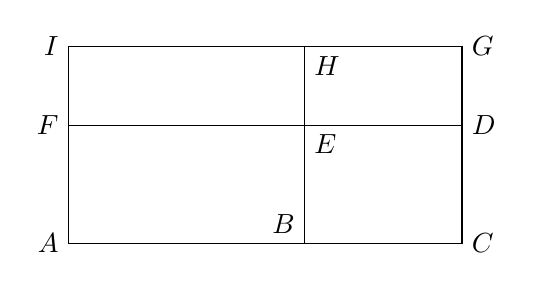
\begin{tikzpicture}
            \draw (0,0) node [left] {$A$}--(3,0) node [above left] {$B$}--(5,0) node [right] {$C$}--(5,1.5) node [right] {$D$}--(3,1.5) node [below right] {$E$}--(0,1.5) node [left] {$F$}--cycle;
            \draw (5,1.5)--(5,2.5) node [right] {$G$} --(3,2.5) node [below right] {$H$} --(0,2.5) node [left] {$I$} --(0,1.5);
            \draw (3,0)--(3,2.5);
        \end{tikzpicture}
    \end{figure}
\end{minipage}

\begin{multicols}{4}
    $22\times 107$

    $34\times 23$

    $41\times 37$

    $81\times 23$
\end{multicols}